\documentclass[a4paper,dvipdfmx,11pt,reqno]{amsart}
\usepackage{amsmath,amsthm,amssymb,mathrsfs,stmaryrd}
\usepackage{bm}
\usepackage[bbgreekl]{mathbbol}
\usepackage{url}
\usepackage{color}
\usepackage{eucal}
\usepackage{slashed}
\usepackage{physics}
\usepackage{graphicx}
\usepackage{tikz}
\usepackage{tikz-cd}
\usetikzlibrary{intersections, calc, arrows, arrows.meta, shadows}
\usepackage[utf8]{inputenc} % for special characters
\usepackage[T1]{fontenc}
\usepackage[backend=biber,style=alphabetic,hyperref=true]{biblatex} % for bib latex
\addbibresource{cf_presentable.bib}
\usepackage{geometry} % margin settings
\geometry{margin=1.0in}
\usepackage{enumitem} % item style
\setlist[enumerate]{itemsep=2pt,parsep=2pt,before={\parskip=2pt}}
\setlist[description]{style=standard}
\usepackage[colorlinks=true,hyperindex, linkcolor=magenta, pagebackref=false, citecolor=cyan,pdfpagelabels]{hyperref} % link colors
\usepackage{cleveref}

\renewcommand{\baselinestretch}{1.1} % change the space between lines

% hiragana yo and oy
\DeclareFontFamily{U}{dmjhira}{}
\DeclareFontShape{U}{dmjhira}{m}{n}{
  <-> dmjhira
}{}
\DeclareFontSubstitution{U}{dmjhira}{m}{n}
\newcommand{\yo}{\text{{\usefont{U}{dmjhira}{m}{n}\symbol{"48}}}}
\newcommand{\oy}{\text{{\reflectbox{\yo}}}}

% math definitions
\DeclareMathOperator{\Ob}{Ob}
\DeclareMathOperator{\Hom}{Hom}
\DeclareMathOperator{\Map}{Map}
\DeclareMathOperator{\myop}{op}
\DeclareMathOperator{\id}{id}
\DeclareMathOperator{\h}{h}
\DeclareMathOperator{\N}{N}
\DeclareMathOperator*{\colim}{colim}
\DeclareMathOperator{\Fun}{Fun}
\DeclareMathOperator{\FunL}{Fun^{L}}
\DeclareMathOperator{\Ind}{Ind}
\DeclareMathOperator{\TwAr}{TwAr}
\renewcommand{\ev}{\mathrm{ev}}

% categories (using mathcal)
\newcommand{\A}{\mathcal{A}}
\newcommand{\B}{\mathcal{B}}
\newcommand{\C}{\mathcal{C}}
\newcommand{\D}{\mathcal{D}}
\newcommand{\E}{\mathcal{E}}
\newcommand{\F}{\mathcal{F}}
\newcommand{\G}{\mathcal{G}}
\newcommand{\I}{\mathcal{I}}
\newcommand{\J}{\mathcal{J}}
\newcommand{\V}{\mathcal{V}}
\newcommand{\W}{\mathcal{W}}
\renewcommand{\H}{\mathcal{H}}
\renewcommand{\O}{\mathcal{O}}
\renewcommand{\P}{\mathcal{P}}
\renewcommand{\S}{\mathcal{S}}

% categories (using math rm)
\newcommand{\An}{\mathrm{An}}
\newcommand{\Cat}{\mathrm{Cat}}
\newcommand{\CAT}{\mathrm{CAT}}
\newcommand{\Kan}{\mathrm{Kan}}
\newcommand{\sSet}{\mathrm{sSet}}
\newcommand{\PrL}{\mathrm{Pr}^{\mathrm{L}}}

% ------------------------------------------------------

% theorem style (using definition style)
\newtheorem{theorem}{Theorem}[section]
\newtheorem*{definition*}{Definition}
\newtheorem*{theorem*}{Theorem}
\newtheorem*{conjecture*}{Conjecture}

\theoremstyle{definition}
\newtheorem{definition}[theorem]{Definition}
\newtheorem{conjecture}[theorem]{Conjecture}
\newtheorem{construction}[theorem]{Construction}
\newtheorem{corollary}[theorem]{Corollary}
\newtheorem{example}[theorem]{Example}
\newtheorem{lemma}[theorem]{Lemma}
\newtheorem{notation}[theorem]{Notation}
\newtheorem{proposition}[theorem]{Proposition}
\newtheorem{question}[theorem]{Question}
\newtheorem{remark}[theorem]{Remark}
\newtheorem{recall}[theorem]{Recall}

% --------------------------------------------------


\title{A Note on Presentable \texorpdfstring{$\infty$}{infty}-Categories}
\author{Keima Akasaka}

\begin{document}

\maketitle 

\begin{abstract}
  We summarize key concepts and results on presentable $\infty$-categories, focusing on their foundational aspects.
\end{abstract} 

% show depth in contents
\setcounter{tocdepth}{2}
\tableofcontents   


\section{Introduction}

We summarize key concepts and results on presentable $\infty$-categories, focusing on their foundational aspects.
We primarily refer to \cite[Chapter 5]{HTT}, but we also make use of \cite{KNP,kerodon,Land}.

Many categories which arise naturally is \textit{large}: 
They have a class of objects.
However, large categories $\C$ can be determined by "small" categories $\C_0$ in some sense:
That is, $\C$ is the equivalent to the category of Ind-objects of $\C_0$.

The aim of this note is to study these "good" large categories, called presentable categories in the setting of $\infty$-categories.

\subsection{Notations}

From here all categories are assumed to be $\infty$-categories.
We let 
\begin{itemize}
  \item $\An$ denote the category of small anima.
  \item $\CAT$ denote the category of (not necessarily small) categories.
  \item $\PrL$ denote the category of presentable categories with left adjoint functors.
\end{itemize}


\section{Yoneda's Lemma}

\subsection{Small Simplicial Sets}

We recall the size conditions of simplicial sets.
Let $\kappa$ be a regular cardinal.

\begin{definition}[\cite{kerodon} \href{https://kerodon.net/tag/03S2}{Definition 03S2}]
  Let $K$ be a simplicial set.
  We will say that $K$ is \textit{$\kappa$-small} if the collection of non-degenerate simplices of $K$ is $\kappa$-small as a set.
  We will say that $K$ is \textit{small} if it is $\kappa$-small for some $\kappa$.
\end{definition}

\begin{definition}[\cite{HTT} Definition 5.4.1.3]
  Let $\C$ be a category.
  We will say that $\C$ is \textit{essentially $\kappa$-small} if there exist a $\kappa$-small category $\C'$ and an equivalence of categories $\C' \to \C$.
  We will say that $\C$ is \textit{essentially small} if it is essentially $\kappa$-small for some $\kappa$.
\end{definition}

\begin{definition}[\cite{HTT} Section 5.4.1]
  Let $\C$ be a category.
  We will say that $\C$ is \textit{locally $\kappa$-small} if, for every pair of objects $X$ and $Y$ of $\C$, the mapping anima $\Map_{\C}(X,Y)$ is essentially $\kappa$-small.
  We will say that $\C$ is \textit{locally small} if it is locally $\kappa$-small for some $\kappa$.
\end{definition}

\begin{definition}[\cite{HTT} Definition 1.2.13.4]
  Let $\C$ be a category, and let $f : K \to \C$ be a diagram of simplicial sets.
  We will refer to an initial object in the category $\C_{f/}$ as a \textit{colimit} for $f$.
  Dually, we will refer to a final object in the category $\C_{/f}$ as a \textit{limit} for $f$.
  If $K$ is $\kappa$-small, then a colimit for $f$ is called \textit{$\kappa$-small}.
\end{definition}

\begin{definition}[\cite{HTT} Definition 5.1.5.7]
  Let $\C$ be a category, and let $\C'$ be a full subcategory of $\C$.
  We will say that $\C'$ is \textit{stable under colimits} if, for every small diagram $f : K \to \C$ which admits a colimit $\overline{f} : K^\triangleright \to \C$, then the map $\overline{f}$ factors through $\C'$. 

  Let $\C$ be a category with small colimits, and let $S$ be a collection of objects of $\C$.
  We will say that $S$ \textit{generates} $\C$ \textit{under colimits} if the following condition is satisfied:
  For every full subcategory $\C'$ of $\C$ containing all elements of $S$, if $\C'$ is stable under colimits, then $\C'$ is equal to $\C$.

  Let $f : S \to \C$ be a functor between categories.
  We will say that $f$ \textit{generates} $\C$ \textit{under colimits} if its image $f(S)$ generates $\C$ under colimits.
\end{definition}

\subsection{The Yoneda embedding}

\begin{definition}[\cite{Land} Definition 4.2.3] \label{Land.def.4.2.3}
  Let $\C$ be a category.
  The \textit{twisted arrow category} $\TwAr(\C)$ of $\C$ is the simplicial set defined by 
  \begin{align*}
    \TwAr(\C)_n := \Hom_{\mathrm{sSet}}([n] \star [n]^{\myop},\C)
  \end{align*}
  for every $n \geq 0$, where $\star$ denotes the join operator.
  % By \href{https://kerodon.net/tag/03JR}{Corollary 03JR}, $\TwAr(\C)$ is a category.
\end{definition}

\begin{remark}
  Let $\C$ be a category.
  Then there are two projections
  \begin{align*}
    s : \TwAr(\C) \to \C
    \quad \text{ and } \quad
    t : \TwAr(\C) \to \C^{\myop} 
  \end{align*}
  which are defined as follows:
  They send each $n$-simplex $\sigma$ of $\TwAr(\C)$ to the composition
  \begin{align*}
    [n] \hookrightarrow [n] \star [n]^{\myop} \xrightarrow{\sigma} \C
    \quad \text{ and } \quad
    [n]^{\myop} \hookrightarrow [n] \star [n]^{\myop} \xrightarrow{\sigma} \C.
  \end{align*}
  respectively.
  Then these projections induce a right fibration 
  \begin{align*}
    (s,t) : \TwAr(\C) \to \C \times \C^{\myop}.
  \end{align*}
  As a consequence, for a category $\C$, $\TwAr(\C)$ is also a category.
\end{remark}

\begin{definition}[\cite{Land} Definition 4.2.5] \label{Land.def.4.2.5}
  Let $\C$ be a category.
  We let 
  \begin{align*}
    \Map_{\C}(-,-) : \C^{\myop} \times \C \to \An 
  \end{align*}
  denote the functor obtained by the straightening of the right fibration $(s,t) : \TwAr(\C) \to \C \times \C^{\myop}$.
\end{definition}

\begin{definition}[\cite{Land} Definition 4.2.9] \label{Land.def.4.2.9}
  Let $\C$ be a category.
  We let 
  \begin{align*}
    \yo : \C \to \Fun(\C^{\myop},\An)
  \end{align*}
  denote the right adjoint functor to $\Map_{\C}(-,-) : \C^{\myop} \times \C \to \An$.
  We will refer to it as the (\textit{contravariant}) \textit{Yoneda embedding}.
  Similarly, we can define the \textit{covariant Yoneda embedding}
  \begin{align*}
    \oy : \C^{\myop} \to \Fun(\C,\An)
  \end{align*}
  as the right adjoint functor to $\Map_{\C}(-,-) : \C^{\myop} \times \C \to \An$.
\end{definition}

There are other constructions of the Yoneda embedding.
These are at least objectwise equivalent to each other.

\begin{remark}
  Recall that there exists the adjunction between the 1-category $\sSet$ of simplicial sets and the 1-category $\Cat_{\Delta}$ of $\sSet$-enriched 1-categories:
  \begin{align*}
    \mathfrak{C} : \sSet \rightleftarrows \Cat_{\Delta} : \N_{\Delta}
  \end{align*}
  where $\mathfrak{C}$ is the \textit{rigidification functor} and $\N_{\Delta}$ is the \textit{simplicial nerve} or \textit{(homotopy) coherent nerve}.
\end{remark}

\begin{construction}[\cite{HTT} Section 5.1.3]
  Let $K$ be a simplicial set.
  We have a simplicial functor 
  \begin{align*}
    \mathfrak{C}[K]^{\myop} \times \mathfrak{C}[K] \to \Kan : (X,Y) \mapsto \mathrm{Sing}|\Map_{\mathfrak{C}[K]}(X,Y)| 
  \end{align*}
  where $\Kan$ is the 1-category of anima.
  The functor $\mathfrak{C}$, in general, does not commute with products, but there is a natural map 
  \begin{align*}
    \mathfrak{C}[K^{\myop} \times K] \to \mathfrak{C}[K]^{\myop} \times \mathfrak{C}[K].
  \end{align*}
  Thus we can obtain a simplicial functor 
  \begin{align*}
    \mathfrak{C}[K^{\myop} \times K] \to \mathfrak{C}[K]^{\myop} \times \mathfrak{C}[K] \to \Kan.
  \end{align*}
  Using the adjunction $\mathfrak{C} \dashv \N_{\Delta}$ and the fact that $\An \simeq \N_{\Delta}(\Kan)$, we get a map of simplicial sets 
  \begin{align*}
    K^{\myop} \times K \to \An.
  \end{align*}
  By further using the adjunction $(K^{\myop} \times -) \dashv \Fun(K^{\myop},-)$, we have a map 
  \begin{align*}
    \yo : K \to \Fun(K^{\myop},\An).
  \end{align*}
  We will refer to the functor $\yo$ constructed above (or more generally, to every functor equivalent to $j$) as the \textit{(contravariant) Yoneda embedding}.
  Similarly, we can define the \textit{(covariant) Yoneda functor} $\oy : K^{\myop} \to \Fun(K,\An)$.
\end{construction}

% \begin{theorem}[\cite{Land} Proposition 4.2.10]
  
% \end{theorem}

\begin{corollary}[\cite{Land} Proposition 4.2.11]
  Let $\C$ be a category.
  Then the Yoneda embedding $\yo$ is fully faithful.
\end{corollary}

\begin{proposition}[\cite{HTT} Proposition 5.1.3.2]
  Let $\C$ be a small category.
  Then the Yoneda embedding $\yo$ preserves small limits which exist in $\C$. 
\end{proposition}

For a category $\C$, $\Fun(\C^{\myop},\An)$ is freely generated by the Yoneda embedding $\yo$ under small colimits.

\begin{theorem}[\cite{HTT} Theorem 5.1.5.6] \label{HTT.5.1.5.6}
  Let $\C$ be a small category, and let $\D$ with small colimits.
  Then the functor $\yo$ induces an equivalence of categories 
  \begin{align*}
    \Fun^{\colim}(\Fun(\C^{\myop},\An),\D) \to \Fun(\C,\D).
  \end{align*}
  The inverse is given by a left Kan extension along $\yo$.
  \[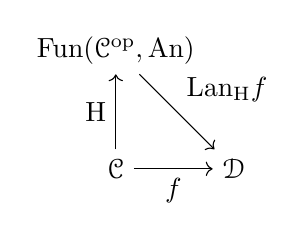
\begin{tikzpicture}[auto,->] 
    \node (al) at (0,1.5) {$\Fun(\C^{\myop},\An)$}; 
    \node (bl) at (0,0) {$\C$}; 
    \node (br) at (1.5,0) {$\D$}; 
    \draw (bl) -- node[swap] {$f$} (br); 
    \draw (bl) -- node {$\yo$} (al);
    \draw (al) -- node {$\mathrm{Lan}_{\yo}f$} (br); 
  \end{tikzpicture}\]
\end{theorem}


\section{The \texorpdfstring{$\infty$}{infty}-Category of Ind-objects}

\subsection{Filtered \texorpdfstring{$\infty$}{infty}-Categories}

\begin{definition}[\cite{HTT} Definition.5.3.1.7]
  Let $\I$ be a category.
  We will say that $\I$ is \textit{$\kappa$-filtered} if, for every $\kappa$-small simplicial set $K$ and every diagram $f : K \to \I$, there exists a map $ \overline{f} : K^\triangleright \to \I$ extending $f$.
  \[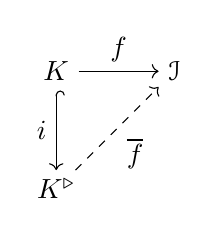
\begin{tikzpicture}[auto] 
    \node (al) at (0,1.5) {$K$}; 
    \node (ar) at (1.5,1.5) {$\I$}; 
    \node (bl) at (0,0) {$K^\triangleright$}; 
    \draw[->] (al) -- node {$f$} (ar); 
    \draw[right hook->] (al) -- node[swap] {$i$} (bl);
    \draw[->,dashed] (bl) -- node[swap] {$\overline{f}$} (ar); 
  \end{tikzpicture}\]
  We will say that $\C$ is \textit{filtered} if it is $\omega$-filtered. 
  If a category $\I$ is $\kappa$-filtered, then a diagram $\I \to \C$ is called \textit{$\kappa$-filtered}.
  Similarly, in this case, a colimit for $\I \to \C$ is called \textit{$\kappa$-filtered}.
\end{definition}

% \begin{remark}
%   Let $\C$ be a 1-category.
%   Then the 1-category $\C$ is $\kappa$-filtered (as a 1-category) if and only if the nerve $\N(\C)$ is $\kappa$-filtered (as a category).
% \end{remark}

\begin{remark}[\cite{HTT} Remark.5.3.1.9]
  Let $\C$ be a category.
  The following conditions are equivalent:
  \begin{enumerate}
    \item The category $\C$ is $\kappa$-filtered.
    \item For every diagram $f : K \to \C$ where $K$ is a $\kappa$-small simplicial set, the category $\C_{f/}$ is not empty.
  \end{enumerate}
  Let $q : \C \to \C'$ be a categorical equivalence.
  It is obvious that $\C_{p/}$ is not empty if and only if $\C_{qp/}$ is not empty.
  Consequently, $\C$ is $\kappa$-filtered if and only if $\C'$ is $\kappa$-filtered. 
\end{remark}

We provide a characterization of $\kappa$-filtered categories using colimit diagrams.

\begin{definition}[\cite{HTT} Definition.5.3.3.1]
  Let $\C$ be a category.
  We will say that $\C$ is \textit{$\kappa$-closed} if every diagram $p : K \to \C$ where $K$ is a $\kappa$-small simplicial set, admits a colimit $\overline{p} : K^\triangleright \to \C$.
\end{definition}

If a category $\C$ is $\kappa$-closed, we can construct $\kappa$-small colimits functionally.

\begin{construction}
  Let $\C$ be a category, and let $K$ be a simplicial set.
  Suppose that every diagram $p : K \to \C$ admits a colimit in $\C$.
  We let $\D$ denote the full subcategory of $\Fun(K^\triangleright,\C)$ spanned by the colimit diagrams.
  \Cite{HTT} Proposition.4.3.2.15 implies that the restriction $\D \to \Fun(K,\C)$ is a trivial fibration.
  Thus it has a section $s : \Fun(K,\C) \to \D$.
  Let $\ev_{\infty} : \Fun(K^\triangleright,\C) \to \C$ be a functor defined by evaluation at the cone point of $K^\triangleright$.
  We will refer to the composition 
  \begin{align*}
    \colim_{K} : \Fun(K,\C) \xrightarrow{s} \D \subseteq \Fun(K^\triangleright,\C) \xrightarrow{\ev_{\infty}} \C
  \end{align*}
  as a \textit{colimit functor} for $p$.
\end{construction}

\begin{proposition}[\cite{HTT} Proposition.5.3.3.3]
  Let $\I$ be a category. 
  The following conditions are equivalent:
  \begin{enumerate}
    \item The category $\I$ is $\kappa$-filtered.
    \item The colimit functor $\colim\limits_{\I} : \Fun(\I,\An) \to \An$ preserves $\kappa$-small limits. 
  \end{enumerate}
\end{proposition}

\subsection{Compact Objects}

\begin{definition}[\cite{HTT} Definition.5.3.4.5]
  Let $\C$ with  $\kappa$-filtered small colimits, and let $f : \C \to \D$ be a functor of categories.
  We will say that $f$ is \textit{$\kappa$-continuous} if it preserves $\kappa$-filtered colimits.

  Let $\C$ be a category with $\kappa$-filtered colimits, and let $X$ be an object of $\C$.
  We will say that $X$ is \textit{$\kappa$-compact} if the functor $\oy_{X} : \C \to \An$ is $\kappa$-continuous.
  We will say that $X$ is \textit{compact} if it is $\omega$-compact. 
\end{definition}

\begin{remark} \label{rem.not_equiv_def_of_compact} 
  In \cite{KNP}, they define a $\kappa$-compact object $X$ as follows: 
  We will say that $X$ is \textit{$\kappa$-compact} if the canonical map 
  \begin{align*}
    \colim_{i \in \I}\Map_{\C}(X,Y_i) \to \Map_{\C}(X,\colim_{i \in \I} Y_i)
  \end{align*}
  is an equivalence for every $\kappa$-filtered small diagram $Y : \I \to \C$.
  % As mentioned in \cref{Gal23.rem.2.67}, however, this definition is not precise.
\end{remark}

\begin{notation}[\cite{HTT} Notation.5.3.4.6]
  Let $\C$ be a category with $\kappa$-filtered colimits.
  We let $\C^{\kappa}$ denote the full subcategory of $\C$ spanned by the $\kappa$-compact objects of $\C$.
\end{notation}

\begin{proposition}[\cite{HTT} Corollary.5.3.4.15] \label{HTT.5.3.4.15}
  Let $\C$ be a category with small $\kappa$-filtered colimits.
  Then $\C^\kappa$ is stable under the $\kappa$-small colimits which exist in $\C$.
  That is, a $\kappa$-small colimit of the $\kappa$-compact objects is $\kappa$-compact. 
\end{proposition}

\begin{proof}
  Let $Y : \I \to \C$ be a $\kappa$-filtered small diagram, and let $X : \J \to \C$ be a $\kappa$-small diagram of $\kappa$-compact objects.
  We want to show that a map
  \begin{align*}
    \colim_{i \in \I}\Map_{\C}(\colim_{j \in \J}X_j, Y_i) \to \Map_{\C}(\colim_{j \in \J}X_j, \colim_{i \in \I}Y_i)
  \end{align*}
  is an equivalence.
  We may write
  \begin{align*}
    \colim_{i \in \I}\Map_{\C}(\colim_{j \in \J}X_j, Y_i) 
    &\simeq \colim_{i \in \I}\lim_{j \in \J}\Map_{\C}(X_j,Y_i) \\
    &\simeq \lim_{j \in \J}\colim_{i \in \I}\Map_{\C}(X_j,Y_i) \\
    &\simeq \lim_{j \in \J}\Map_{\C}(X_j,\colim_{i \in \I}Y_i) \\
    &\simeq \Map_{\C}(\colim_{j \in \J}X_j,\colim_{i \in \I}Y_i).
  \end{align*}
\end{proof}

% \begin{remark} \label{rem.mapping_space_functor_1} 
%   If we use the (non-precise) definition of \cref{rem.not_equiv_def_of_compact}, we can prove \cref{HTT.5.3.4.15} simply but only intuitively:
% \end{remark}

\subsection{The \texorpdfstring{$\infty$}{infty}-Category of Ind-objects}

We showed that the category $\Fun(\C^{\myop},\An)$ is freely generated by the functor $\yo$ under small colimits (\cref{HTT.5.1.5.6}).
We next consider the analogue situation only under $\kappa$-filtered small colimits.

\begin{definition}[\cite{HTT} Section.5.3.5] % below Rem.5.3.5.6
  Let $\C$ be a small category.
  We define $\Ind_{\kappa}(\C)$ as the smallest full subcategory of $\Fun(\C^{\myop},\An)$ which contains the image of $\yo$ and is stable under $\kappa$-filtered colimits.
  When $\kappa = \omega$, we will write $\Ind(\C)$ for $\Ind_{\kappa}(\C)$.
  We will refer to $\Ind(\C)$ as the category of \textit{Ind-objects} of $\C$.
\end{definition}

If a category $\C$ admits $\kappa$-small colimits, we can easily characterize the category $\Ind_{\kappa}(\C)$.

\begin{proposition}[\cite{HTT} Corollary.5.3.5.4] \label{HTT.5.3.5.4}
  Let $\C$ be a small category with $\kappa$-small colimits, and let $F : \C^{\myop} \to \An$ be a functor.
  The following conditions are equivalent:
  \begin{enumerate}
    \item The functor $F$ belongs to $\Ind_{\kappa}(\C)$.
    \item The functor $F$ preserves $\kappa$-small limits.
  \end{enumerate} 
  In particular, if $\C$ admits $\kappa$-small colimits, $\Ind_{\kappa}(\C)$ admits small limits.
\end{proposition}

\begin{proposition}[\cite{HTT} Proposition.5.3.5.5] \label{HTT.5.3.5.5}
  Let $\C$ be a small category, and let $\yo : \C \to \Ind_{\kappa}(\C)$ be the Yoneda embedding.
  Then for every object $X$ of $\C$, $\yo X$ is $\kappa$-compact of $\Ind_{\kappa}(\C)$.
\end{proposition}

\begin{proof}
  Let $Y : \I \to \Fun(\C^{\myop},\An)$ be a $\kappa$-filtered small diagram.
  We may write 
  \begin{align*}
    \colim_{i \in \I}\Map_{\Ind_{\kappa}(\C)}(\yo X,Y_i) 
    &\simeq \colim_{i \in \I}\Map_{\Fun(\C^{\myop},\An)}(\yo X,Y_i) \\
    &\simeq \colim_{i \in \I}(Y_i(X)) \\
    &\simeq (\colim_{i \in \I} Y_i)(X) \\
    &\simeq \Map_{\Fun(\C^{\myop},\An)}(\yo X,\colim_{i \in \I}Y_i) \\
    &\simeq \Map_{\Ind_{\kappa}(\C)}(\yo X,\colim_{i \in \I}Y_i).
  \end{align*}
\end{proof}

% \begin{proof}
%   It suffices to show that $\yo_{\yo(X)} : \Ind_{\kappa}(\C)^{\myop} \to \An$ preserves $\kappa$-filtered colimits, where $\yo : \Ind_{\kappa}(\C) \to \Fun(\Ind_{\kappa}(\C)^{\myop}, \An)$.
%   The functor $\yo(X) :  \Ind_{\kappa}(\C)^{\myop} \to \An$ is equivalent to the composition 
%   \begin{align*}
%     \Ind_{\kappa}(\C) \subseteq \Fun(\C^{\myop},\An) \xrightarrow{\ev_{X}} \An.
%   \end{align*}
%   The first inclusion preserves $\kappa$-filtered colimits, since $\Ind_{\kappa}(\C)$ is stable under $\kappa$-filtered colimits.
%   It follows from \cite{HTT} Proposition.5.1.2.2 that the second map preserves all small colimits.
% \end{proof}

% \begin{remark} \label{rem.another_proof_of_HTT.5.3.5.5} \label{rem.mapping_space_functor_2}
%   As \cref{rem.mapping_space_functor_1}, we can intuitively show \cref{HTT.5.3.5.5}.
%   \Cite{HTT} Proposition.5.3.4.13 implies it suffices to prove that for every object $X$ of $\C$, $jX$ is $\kappa$-compact in $\An$.
% \end{remark}

We show that the category $\Ind_{\kappa}(\C)$ is freely generated by $\C$ under $\kappa$-filtered colimits.

\begin{proposition}[\cite{HTT} Proposition.5.3.5.10]
  Let $\C$ be a small category, and let $\D$ be a category with small $\kappa$-filtered colimits.
  Then the functor $\yo : \C \to \Ind_{\kappa}(\C)$ induces an equivalence of categories 
  \begin{align*}
    \Fun^{\colim_{\kappa\text{-filt}}}(\Ind_{\kappa}(\C),\D) \to \Fun(\C,\D). 
  \end{align*}
  The inverse is given by a left Kan extension (\cite{HTT} Lemma.5.3.5.8). 
  \[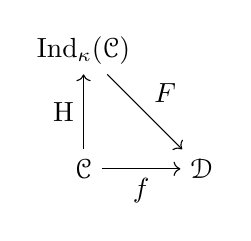
\begin{tikzpicture}[auto,->] 
    \node (al) at (0,1.5) {$\Ind_{\kappa}(\C)$}; 
    \node (bl) at (0,0) {$\C$}; 
    \node (br) at (1.5,0) {$\D$}; 
    \draw (bl) -- node[swap] {$f$} (br); 
    \draw (bl) -- node {$\yo$} (al);
    \draw (al) -- node {$F$} (br); 
  \end{tikzpicture}\]
  We will refer to this inverse as the \textit{$\Ind_{\kappa}$-extension} $F : \Ind_{\kappa}(\C) \to \D$ of the functor $f : \C \to \D$. 
\end{proposition}

The following proposition will be useful throughout this paper.

\begin{proposition}[\cite{HTT} Proposition.5.3.5.11] \label{HTT.5.3.5.11}
  Let $f : \C \to \D$ be a functor between categories.
  Suppose that $\D$ admits small $\kappa$-filtered colimits.
  Let $F : \Ind_{\kappa}(\C) \to \D$ be the $\Ind_{\kappa}$-extension of $f$.
  Then
  \begin{enumerate}
    \item If the functor $f$ is fully faithful and its essential image consists of $\kappa$-compact objects of $\D$, then $F$ is fully faithful.
    \item If additionally to (1), the image of $f$ generate $\D$ under $\kappa$-filtered colimits, then $F$ is an equivalence.
  \end{enumerate}
\end{proposition}

\begin{proof}
  (1):
  Let $X$ and $Y$ be objects of $\Ind_{\kappa}(\C)$.
  From the definition of $\Ind_{\kappa}(\C)$, $X$ and $Y$ are of the form 
  \begin{align*}
    X \simeq \colim_{i \in \I}\yo X_i ,~~\text{ and } Y \simeq \colim_{j \in \J}\yo Y_j 
  \end{align*}
  for some filtered diagrams $\I \to \C$ and $\J \to \C$.
  We want to show that a map
  \begin{align*}
    \Map_{\Ind_{\kappa}(\C)}(X,Y) \to \Map_{\D}(F(X),F(Y))
  \end{align*}
  is an equivalence.
  We may write 
  \begin{align*}
    \Map_{\Ind_{\kappa}(\C)}(X,Y) 
    &\simeq \Map_{\Ind_{\kappa}(\C)}(\colim_{i \in \I}\yo X_i,\colim_{j \in \J}\yo Y_j) \\
    &\simeq \lim_{i \in \I}\colim_{j \in \J}\Map_{\Ind_{\kappa}(\C)}(\yo X_i,\yo Y_j) \\
    &\simeq \lim_{i \in \I}\colim_{j \in \J}\Map_{\C}(X_i,Y_j) \\
    &\simeq \lim_{i \in \I}\colim_{j \in \J}\Map_{\D}(f(X_i),f(Y_j)) \\
    &\simeq \Map_{\D}(\colim_{i \in \I}f(X_i),\colim_{j \in \J}f(Y_j)) \\
    &\simeq \Map_{\D}(\colim_{i \in \I}F(\yo X_i),\colim_{j \in \J}F(\yo Y_j)) \\
    &\simeq \Map_{\D}(F(\colim_{i \in \I}\yo X_i),F(\colim_{j \in \J}\yo Y_j)) \\
    &\simeq \Map_{\D}(F(X),F(Y)).
  \end{align*}
  
  (2): 
  The essential image of $F$ contains the image of $f$ and is stable under small $\kappa$-filtered colimits.
  Thus $F$ is essentially surjective.
\end{proof}

% \begin{remark} \label{rem.mapping_space_functor_3}
%   As \cref{rem.mapping_space_functor_1}, we can intuitively show \cref{HTT.5.3.5.11}.
% \end{remark}

\begin{proposition}[\cite{HTT} Proposition.5.3.5.14] \label{HTT.5.3.5.14}
  Let $\C$ be a small category with $\kappa$-small colimits.
  Then the functor $\yo : \C \to \Ind_{\kappa}(\C)$ preserves $\kappa$-small colimits which exist in $\C$.
\end{proposition}

\begin{proof}
  Let $X : \I \to \C$ be a $\kappa$-small diagram.
  We want to show that a map
  \begin{align*}
    \colim_{i \in \I} \yo X_i 
    \to \yo \colim_{i \in \I} X_i 
  \end{align*}
  is an equivalence.
  By Yoneda's lemma, it is enough to show that a map 
  \begin{align*}
    \Map_{\Ind_\kappa(\C)}(\yo \colim_{i \in \I} X_i,F) 
    \to \Map_{\Ind_\kappa(\C)}(\colim_{i \in \I} \yo X_i,F)
  \end{align*}
  is an equivalence for every functor $F : \C^{\myop} \to \An$.
  We have equivalences
  \begin{align*}
    \Map_{\Ind_\kappa(\C)}(\yo \colim_{i \in \I} X_i,F)
    &\simeq F(\colim_{i \in \I} X_i) \\
    \Map_{\Ind_\kappa(\C)}(\colim_{i \in \I} \yo X_i,F)
    &\simeq \lim_{i \in \I}\Map_{\Ind_\kappa(\C)}(\yo X_i,F) 
    \simeq \lim_{i \in \I}F(X_i).
  \end{align*}
  Since $F$ preserves $\kappa$-small limit from \cref{HTT.5.3.5.4}, these are equivalent.
\end{proof}

% \begin{remark} \label{rem.mapping_space_functor_4}
%   As \cref{rem.mapping_space_functor_1}, we can intuitively show \cref{HTT.5.3.5.14}.
% \end{remark}

\begin{corollary}[\cite{HTT} Example.5.3.6.8] \label{HTT.5.3.6.8}
  Let $\C$ be a small category with $\kappa$-small colimits.
  Then $\Ind_{\kappa}(\C)$ admits small colimits. 
  Moreover, for every category $\D$ with small colimits, the restriction along $\yo$ induces an equivalence of categories
  \begin{align*}
    \Fun^{\colim}(\Ind_{\kappa}(\C),\D) \to \Fun^{\colim_{\kappa\text{-filt}}}(\C,\D).
  \end{align*}
\end{corollary}

\begin{proof}
  Every small colimit can be written as a $\kappa$-filtered colimit of $\kappa$-small colimits.
  It follows from the definition of $\Ind_{\kappa}(\C)$ and \cref{HTT.5.3.5.14}.
\end{proof}


\section{Presentable \texorpdfstring{$\infty$}{infty}-Categories}

\subsection{Accessible \texorpdfstring{$\infty$}{infty}-Categories}

\begin{definition}[\cite{HTT} Definition.5.4.2.1]
  Let $\C$ be a category.
  We will say that $\C$ is \textit{$\kappa$-accessible} if there exist a small category $\C^0$ and an equivalence of categories
  \begin{align*}
    \Ind_{\kappa}(\C^0) \to \C.
  \end{align*}
  We will say that $\C$ is \textit{accessible} if it is $\kappa$-accessible for some $\kappa$. 
\end{definition}

\begin{definition}[\cite{HTT} Definition.5.4.2.5]
  Let $f : \C \to \D$ be a functor between categories.
  We will say that $f$ is \textit{accessible} if it is $\kappa$-continuous for some $\kappa$.
\end{definition}

We can characterize accessible categories as follows:

\begin{proposition}[\cite{HTT} Proposition.5.4.2.2]
  Let $\C$ be a category.
  Then $\C$ is accessible if and only if the following conditions are satisfied:
  \begin{enumerate}
    \item The category $\C$ is locally small, and the category $\C^{\kappa}$ is essentially small.
    \item The category $\C$ admits $\kappa$-filtered small colimits.
    \item The category $\C^{\kappa}$ generates $\C$ under $\kappa$-filtered small colimits.
  \end{enumerate}
\end{proposition}

\subsection{Presentable \texorpdfstring{$\infty$}{infty}-Categories}

\begin{definition}[\cite{HTT} Definition.5.5.0.1]
  Let $\C$ be a category.
  We will say that $\C$ is \textit{presentable} if $\C$ is accessible and admits small colimits.
\end{definition}

\begin{theorem}[\cite{HTT} Theorem.5.5.1.1] \label{HTT.5.5.1.1}
  Let $\C$ be a category.
  The following conditions are equivalent:
  \begin{enumerate}
    \item The category $\C$ is presentable.
    \item The category $\C$ is accessible, and the full subcategory $\C^{\kappa}$ admits $\kappa$-small colimits for every regular cardinal $\kappa$.
    \item There exists a regular cardinal $\kappa$ such that $\C$ is $\kappa$-accessible, and $\C^{\kappa}$ admits $\kappa$-small colimits.
    \item There exist a regular cardinal $\kappa$, a small category $\D$ which admits $\kappa$-small colimits, and an equivalence of categories $\Ind_{\kappa}(\D) \to \C$.
    \item There exists a small category $\D$ such that $\C$ is an accessible localization of $\Fun(\D^{\myop},\An)$.
  \end{enumerate}
\end{theorem}

\begin{remark}
  Let $\C$ be a presentable category.
  It follows from \cref{HTT.5.3.5.4,HTT.5.5.1.1} that $\C$ admits small limits.  
\end{remark}

The following theorem is the \textit{adjoint functor theorem} in the setting of $\infty$-categories.

\begin{theorem}[\cite{HTT} Corollary.5.5.2.9] \label{HTT.5.5.2.9}
  Let $F : \C \to \D$ be a functor between presentable categories. 
  Then
  \begin{enumerate}
    \item The functor $F$ has a right adjoint if and only if $F$ preserves small colimits.
    \item The functor $F$ has a left adjoint if and only if $F$ is accessible and preserves small limits.
  \end{enumerate}
\end{theorem}

\Cref{HTT.5.5.2.9} suggests that an appropriate concept of morphisms between presentable categories are described by pairs of adjoint functors.

\begin{definition}[\cite{HTT} Definition.5.5.3.1]
  Let $\PrL \subseteq \CAT$ denote the (very big) category whose objects are presentable categories and whose morphisms are left adjoint (or colimit-preserving) functors.
\end{definition}

The next results imply that the category $\PrL$ is stable under various categorical constructions.

\begin{example}
  The category $\An$ is presentable.

  If $\C$ is a small category, then the category $\Fun(\C^{\myop},\An)$ is presentable (\cite{HTT} Proposition.5.5.3.6).

  If $\C$ is a small category, then the categories $\C_{/f}$ and $\C_{f/}$ are presentable for every diagram $f : K \to \C$, where $K$ is a small simplicial set. (\cite{HTT} Proposition.5.5.3.10, 5.5.3.11).
\end{example}

\begin{proposition}[\cite{HTT} Proposition.5.5.3.6] \label{HTT.5.5.3.6}
  Let $\C$ be a small category, and let $\D$ be a presentable category.
  Then the category $\Fun(\C,\D)$ is presentable.
\end{proposition}

\begin{proposition}[\cite{HTT} Proposition.5.5.3.8] \label{HTT.5.5.3.8}
  Let $\C$ and $\D$ be presentable categories.
  Then the category $\Fun^{\colim}(\C,\D)$ is presentable.
\end{proposition}

\Cref{HTT.5.5.3.8} implies that the category $\Fun^{\colim}(\C,\D)$ can be regarded as an internal mapping object in $\PrL$.
We can show that there exists a \textit{tensor product} $\otimes$ left adjoint to this functor.
The operation $\otimes$ endows a symmetric monoidal structure on $\PrL$.
\Cref{HTT.5.5.3.8} shows that this symmetric monoidal structure is closed.

% \begin{lemma}[\cite{HTT} Remark.5.5.3.7] \label{HTT.5.5.3.7}
%   Let $\C$ be a small category.
%   Then the category $\Fun(\C^{\myop},\An)$ is presentable.
%   The Yoneda embedding $\C \to \Fun(\C^{\myop},\An)$ is left adjoint to the inclusion $\PrL \subseteq \CAT$.
% \end{lemma}

\begin{proposition}[\cite{HTT} Proposition.5.5.3.13] \label{HTT.5.5.3.13}
  The category $\PrL$ admits small colimits, and the inclusion $\PrL \subseteq \CAT$ preserves small limits.
\end{proposition}

\subsection{Compactly Generated \texorpdfstring{$\infty$}{infty}-Categories}

\begin{definition}[\cite{HTT} Definition.5.5.7.1]
  Let $\C$ be a category.
  We will say that $\C$ is \textit{$\kappa$-compactly generated} if $\C$ is presentable and $\kappa$-accessible.
  We will say that $\C$ is \textit{compactly generated} if it is $\omega$-compactly generated.
\end{definition}

\begin{proposition}[\cite{HTT} Section.5.5.7]
  Let $\C$ be a category.
  The following conditions are equivalent:
  \begin{enumerate}
    \item The category $\C$ is $\kappa$-compactly generated.
    \item There exist a small category $\D$ which admits $\kappa$-small colimits and an equivalence $\Ind_{\kappa}(\D) \to \C$. 
    Moreover, we can choose $\D$ to be the full subcategory $\C^{\kappa}$ of $\kappa$-compact objects of $\C$.
  \end{enumerate}
\end{proposition}
 
% \begin{remark}
%   Since inclusion $\C^{\kappa} \subseteq \C$ satisfies the assumption of \cref{HTT.5.3.5.11} (1), then the $\Ind_{\kappa}$-extension $\Ind_{\kappa}(\C^{\kappa}) \to \C$ of the inclusion $\C^{\kappa} \subseteq \C$ is automatically fully faithful.
%   Thus we can say the condition (2) as follows:
%   \begin{itemize}
%     \item[(2')] There exists a category $\D$ which admits small colimits and $\D^{\kappa}$ is small, and an equivalence $\C \simeq \Ind_{\kappa}(\D^{\kappa})$.
%   \end{itemize}
% \end{remark}

% \begin{remark}
%   By the above remark, we can define presentable categories by compactly generated categories:
%   Let $\C$ be a category.
%   The following conditions are equivalent:
%   \begin{enumerate}
%     \item The category $\C$ is presentable.
%     \item The category $\C$ satisfies (2)' and admits small colimits.
%   \end{enumerate}
% \end{remark}

% \begin{lemma}[\cite{KNP} Lemma.2.1.15]
%   Let $\C$ be a category.
%   The following conditions are equivalent:
%   \begin{enumerate}
%     \item The category $\C$ is $\kappa$-compactly generated.
%     \item Every object of $\C$ can be written as a small colimit of $\kappa$-compact objects.
%   \end{enumerate}
% \end{lemma}

\begin{proposition}[\cite{HTT} Proposition.5.5.7.2]
  Let $\C$ and $\D$ be categories with $\kappa$-filtered colimit, and $L : \C \rightleftarrows \D : R$ be an adjunction.
  Then 
  \begin{enumerate}
    \item If the functor $R$ is $\kappa$-continuous, then the functor $L$ preserves $\kappa$-compact objects.
    \item If $\C$ is $\kappa$-accessible and the functor $L$ preserves $\kappa$-compact objects, then the functor $R$ is $\kappa$-continuous.
  \end{enumerate}
\end{proposition}

% \begin{notation}[\cite{HTT} Notation.5.5.7.7]
%   We let $\PrL_{\kappa}$ denote the (non full) subcategory of $\CAT$ whose objects are $\kappa$-compactly generated categories and whose morphisms are functors which preserve small colimits and $\kappa$-compact objects.

%   We let $\CAT^{\mathrm{Rex}(\kappa)}$ denote the (non full) subcategory of $\CAT$ whose objects are categories with $\kappa$-small colimits and whose objects are functors which preserve $\kappa$-small colimits. 
% \end{notation}

% \begin{proposition}[\cite{HTT} Proposition.5.5.7.10]
%   If $\kappa > \omega$, then 
% \end{proposition}

% \begin{proposition}[\cite{HTT} Proposition.5.5.7.6]
%   The category $\PrL_{\kappa}$ admits small colimits, and the inclusion $\PrL_{\kappa} \subseteq \PrL$ preserves small colimits.
% \end{proposition}

% \subsection{Localization and Local Objects}

% We show that every presentable category arises from a Bousfield localization.

% \begin{definition}[\cite{HTT} Definition.5.2.7.2]
%   Let $f : \C \to \D$ be a functor between categories.
%   We will say that $f$ is a \textit{Bousfield localization} if it has a fully faithful right adjoint functor. 
  
%   In this case, we will say that $\D$ is a \textit{Bousfield localization} of $\C$.
%   We will refer to a composition $L=gf : \C \to \C$ as a \textit{Bousfield localization functor} if it arises in this way.
% \end{definition}

% \begin{proposition}[\cite{HTT} Definition.5.2.7.12]
%   Let $\C$ be a category, and let $L : \C \to \C$ be a localization functor with essential image $L\C$.
%   Let $S$ be a collection of the morphisms $f$ in $\C$ such that $Lf$ is an equivalence.
%   Then for every category $\D$, the functor $L$ induces a fully faithful functor 
%   \begin{align*}
%     \Fun(L\C,\D) \to \Fun(\C,\D).
%   \end{align*}
%   Moreover, its essential image consists of the functors $F : \C \to \D$ such that $Ff$ is an equivalence in $\D$ for every morphism $f$ in $S$.
% \end{proposition}


\printbibliography


\end{document}

% \begin{remark}[\cite{Gal23} Remark.2.67] \label{Gal23.rem.2.67}
%   Let $\C$ be a category.
%   We note that the functor $\C^{\myop} \times \C \to \An$ constructed above is pointwise equivalent to the mapping anima in $\C$, but not equal.
%   In many cases of $\infty$-categories, the mapping space bifunctor will be defined. 
%   Therefore, some notions are sometimes defined and proved using this mapping bifunctor 
%   (see \cref{rem.not_equiv_def_of_compact,rem.mapping_space_functor_1,rem.mapping_space_functor_2,rem.mapping_space_functor_3,rem.mapping_space_functor_4}) 
%   instead of the Yoneda embedding. 
%   However, rigorous statements should be based on the argument using the Yoneda embedding.
% \end{remark}